\chapter{Phương pháp và mô hình đề xuất }
\label{chapter3}
\section{Tổng quan hệ thống}


Kế thừa những điểm tốt trong kiến trúc của DeepExploit \cite{takaesudeepexploit}, tổng quan mô hình đề xuất học tăng cường sâu gồm:

\begin{itemize}
    \item Một server làm nhiệm vụ train cho agent
    \item State của môi trường bao gồm 5 thuộc tính: OS type, product name on port, product version, exploit module of product, target type of module
    \item Một action chính là payload thực hiện lên trên môi trường đặt tại server train
    \item Một hàm reward có nhiệm vụ "cho điểm" nếu action được đánh giá tốt.
\end{itemize}
được thể hiện trong \textbf{Hình \ref{fig:chap3-rlauto-pentest}}. Học tăng cường sâu là sự kết hợp của học tăng cường và học sâu. Trong thực tế, phần "sâu" ở đây là về việc sử dụng mạng nơ-ron với các tham số trọng số $\theta$ để xấp xỉ hàm giá trị $Q(s, a)$ trong quá trình đào tạo agent RL.

\begin{figure}[!h]
    \centering
    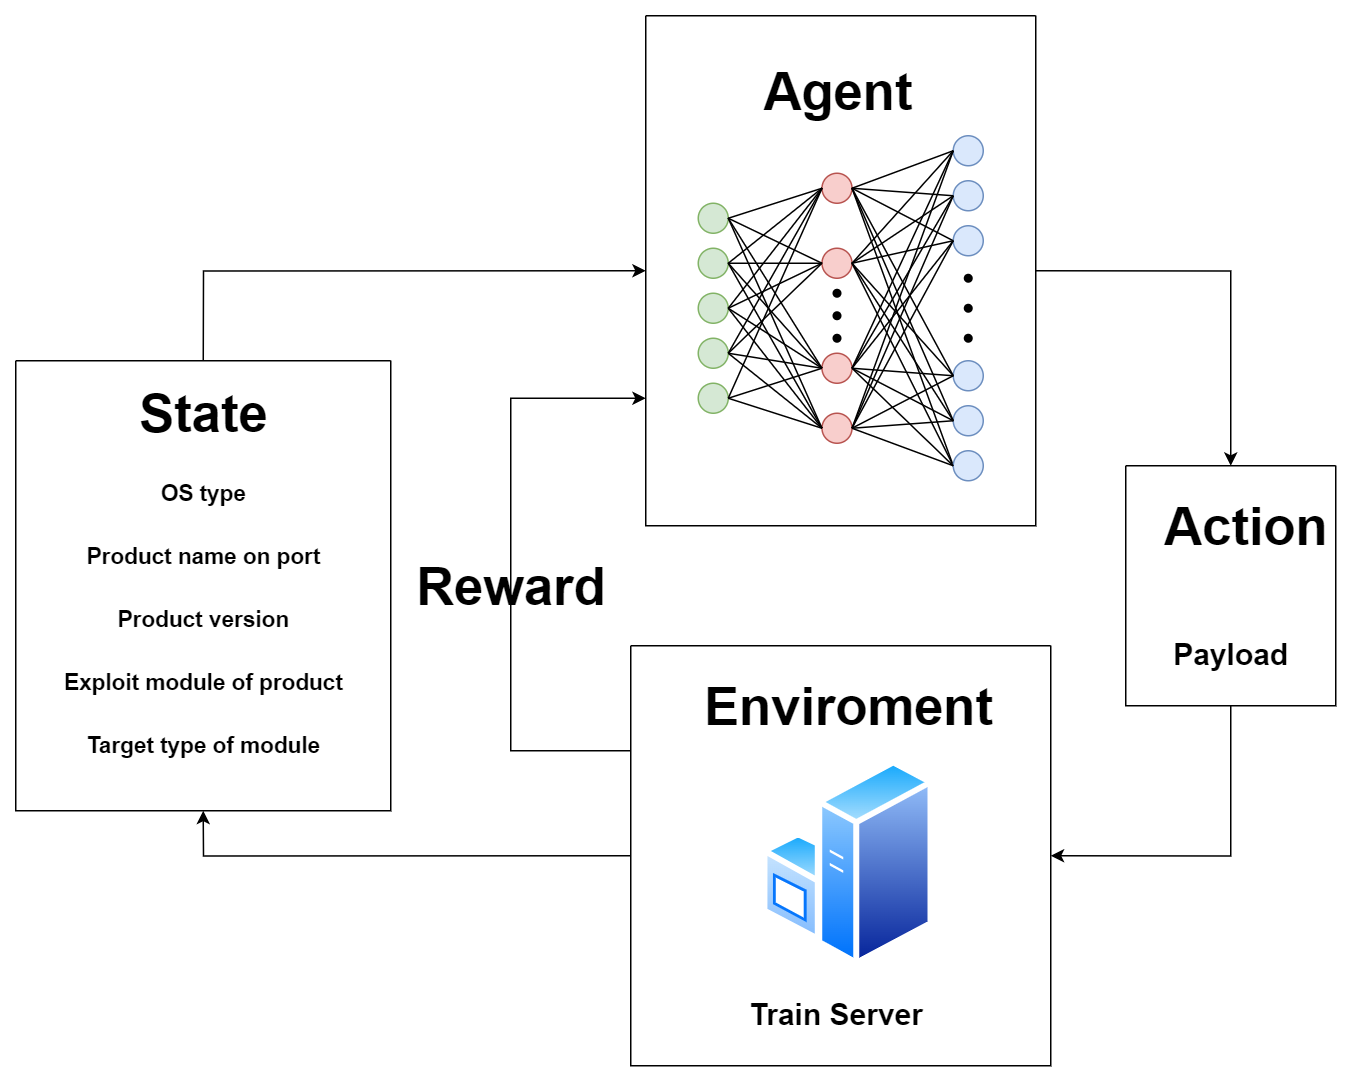
\includegraphics[scale=0.3]{graphics/chapter-3/chap3-rlauto-pentest.png}
    \caption{Kiến trúc tổng thể }
    \label{fig:chap3-rlauto-pentest}
\end{figure}


\section{Mô hình Quyết định Markov (MDP)}

Một vấn đề đặt ra là quá trình học tăng cường tác động liên tục qua lại với môi trường huấn luyện nó. Để chỉ định các ràng buộc (mà biến thiên qua quá trình huấn luyện) giữa môi trường với agent, mỗi vòng lặp huấn luyện sử dụng mô hình quyết định Markov (MDP) \cite{levin1998using}.

MDP là một khung lý thuyết thường được sử dụng để mô tả các tình huống quyết định trong môi trường chưa xác định và biểu diễn quá trình ra quyết định trong điều kiện không hoàn hảo. Nó gồm các thành phần chính như trạng thái của môi trường, không gian vector hoạt động và hàm reward. Trạng thái là những nhiều diễn tình trạng môi trường hiện tại, hành động là những lựa chọn mà agent có thể thực hiện để thay đổi trạng thái, trong khi hàm reward thực hiện đánh giá hiệu quả của hành động đó.

Một điểm quan trọng trong MDP là tính chất Markov, có nghĩa là trạng thái tiếp theo chỉ phụ thuộc vào trạng thái hiện tại và hành động được thực hiện, không phụ thuộc vào quá khứ. Điều này giúp giảm đáng kể kích thước của không gian trạng thái, làm cho quyết định trở nên hiệu quả hơn.

\begin{itemize}
    \item \textbf{Trạng thái} $s$ bao gồm 5 thuộc tính như sau:
    
        \begin{itemize}
            \item OS type
            \item Product name on port
            \item Product version
            \item Exploit module of product
            \item Target type of module on Metasploit framework
        \end{itemize}

    Dựa trên trạng thái $s$, agent RL thực hiện 1 hành động $a$ để khai thác các lỗ hổng. Và \textbf{hành động} $a =$ \{Excellent, Great, Good\}  là một vector của 3 loại đánh giá trong Metasploit.
    \item \textbf{Phần thưởng} $r$ được xác định là tích cực nếu payload được chọn thành công và tiêu cực nếu payload được chọn thất bại. Agent được huấn luyện để tối đa hóa kỳ vọng của phần thưởng tích lũy có chiết khấu dựa trên công thức \textbf{(\ref{reward})}.
    \begin{equation}
        R = \sum^{T}_{t=1} \gamma^{t-1} r_t  
        \label{reward}
    \end{equation}
    với $\gamma \in (0, 1]$  hệ số chiết khấu tương lai.
    \item \textbf{Chính sách} $\pi$ là một hàm để quyết định hành động $a$ có sẵn cho trạng thái $s$.
    \item \textbf{Hàm giá trị} $V_{\pi}(s)$ ước tính mức độ tốt của việc thực hiện một hành động $a$ cụ thể theo chính sách $\pi$ trong trạng thái $s$.
    \begin{equation}
        V_{\pi}(s) = E\{\sum^{\infty}_{t=0} \gamma^{t} r_t  \}
        \label{vvalue}
    \end{equation}
    \item \textbf{Hàm giá trị hành động tối ưu} $Q^*(s_t, a)$ được thể hiện trong Công thức \textbf{(\ref{qvalue})} ước tính phần thưởng kỳ vọng của việc thực hiện một hành động $a$ tại $t^{th}$ trạng thái $s_t$. 
    \begin{equation}
        Q^*(s_t, a) = E\{r_{t} + \gamma \max_{a'} Q^*(s_{t+1},a')\}
        \label{qvalue}
    \end{equation}
\end{itemize}

\section{Huấn luyện tác nhân Học tăng cường sâu}

\subsection{Thuật toán Asynchronous Advantage Actor Critic - A3C}

Bản chất của học tăng cường (RL) dựa trên nguyên tắc phần thưởng, tức là thử - sai và điều chỉnh. Trong số nhiều mô hình RL, A3C là một policy gradient algorithm có chính sách $\pi(s_t,a;\theta)$ và hàm ước tính giá trị $V(s_t;\theta)$. Ý nghĩa của 3 chữ cái A trong thuật toán A3C \cite{mnih2016asynchronous} được mô tả như sau:

\begin{itemize}
    \item \textbf{Advantage:} một đặc điểm nơi thay vì sử dụng giá trị phần thưởng có chiết khấu $\gamma$ để cho agent biết hành động nào tốt trong tương lai, chúng ta sử dụng giá trị của hàm \textit{"advantage"}. Điều này agent RL học các phần thưởng tốt hơn. Giá trị \textit{advantage} được cho bởi biểu thức: $A = Q(s,a) - V(s)$
    \item \textbf{Actor-Critic:} một đặc điểm là A3C kết hợp dự đoán hàm giá trị $V$ cũng như chính sách tối ưu $\pi(s)$ (tức là phân phối xác suất của không gian hành động). Agent học sử dụng giá trị của hàm giá trị (Critic) để cập nhật hàm chính sách (Actor). 
    \item \textbf{Asynchronous:} A3C sử dụng nhiều agent, mỗi agent có các tham số mạng nơ-ron riêng và một bản sao của môi trường. Những agent này tương tác với môi trường của chúng một cách không đồng bộ, học với mỗi tương tác. Mỗi khi chúng tích lũy được "kinh nghiệm", nó sẽ đóng góp "kiến thức" vào \textit{Mạng toàn cục}, cũng chính là mạng quản lý chúng. Như vậy, thay vì chỉ học bằng một agent, các agent học song song và tựu trung, mô hình sẽ được huấn luyện nhanh hơn.
\end{itemize}

Cấu trúc của mô hình A3C với 2 agent học song song thể hiện trong \textbf{Hình \ref{fig:chap3-a3cParallel}}.

\begin{figure}[!h]
    \centering
    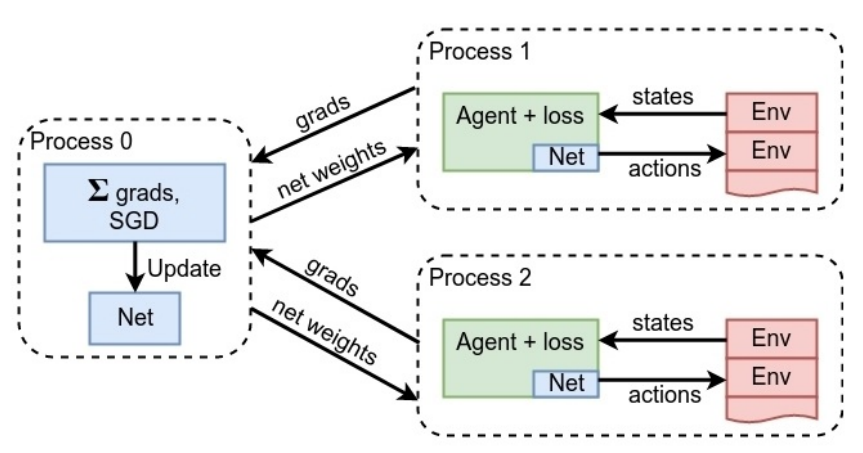
\includegraphics[scale=0.8]{graphics/chapter-3/chap3-a3cParallel.PNG}
    \caption{Mô hình A3C với hai agent học song song}
    \label{fig:chap3-a3cParallel}
\end{figure}


\subsection{Huấn luyện  agent với thuật toán A3C}

\begin{figure}[!h]
    \centering
    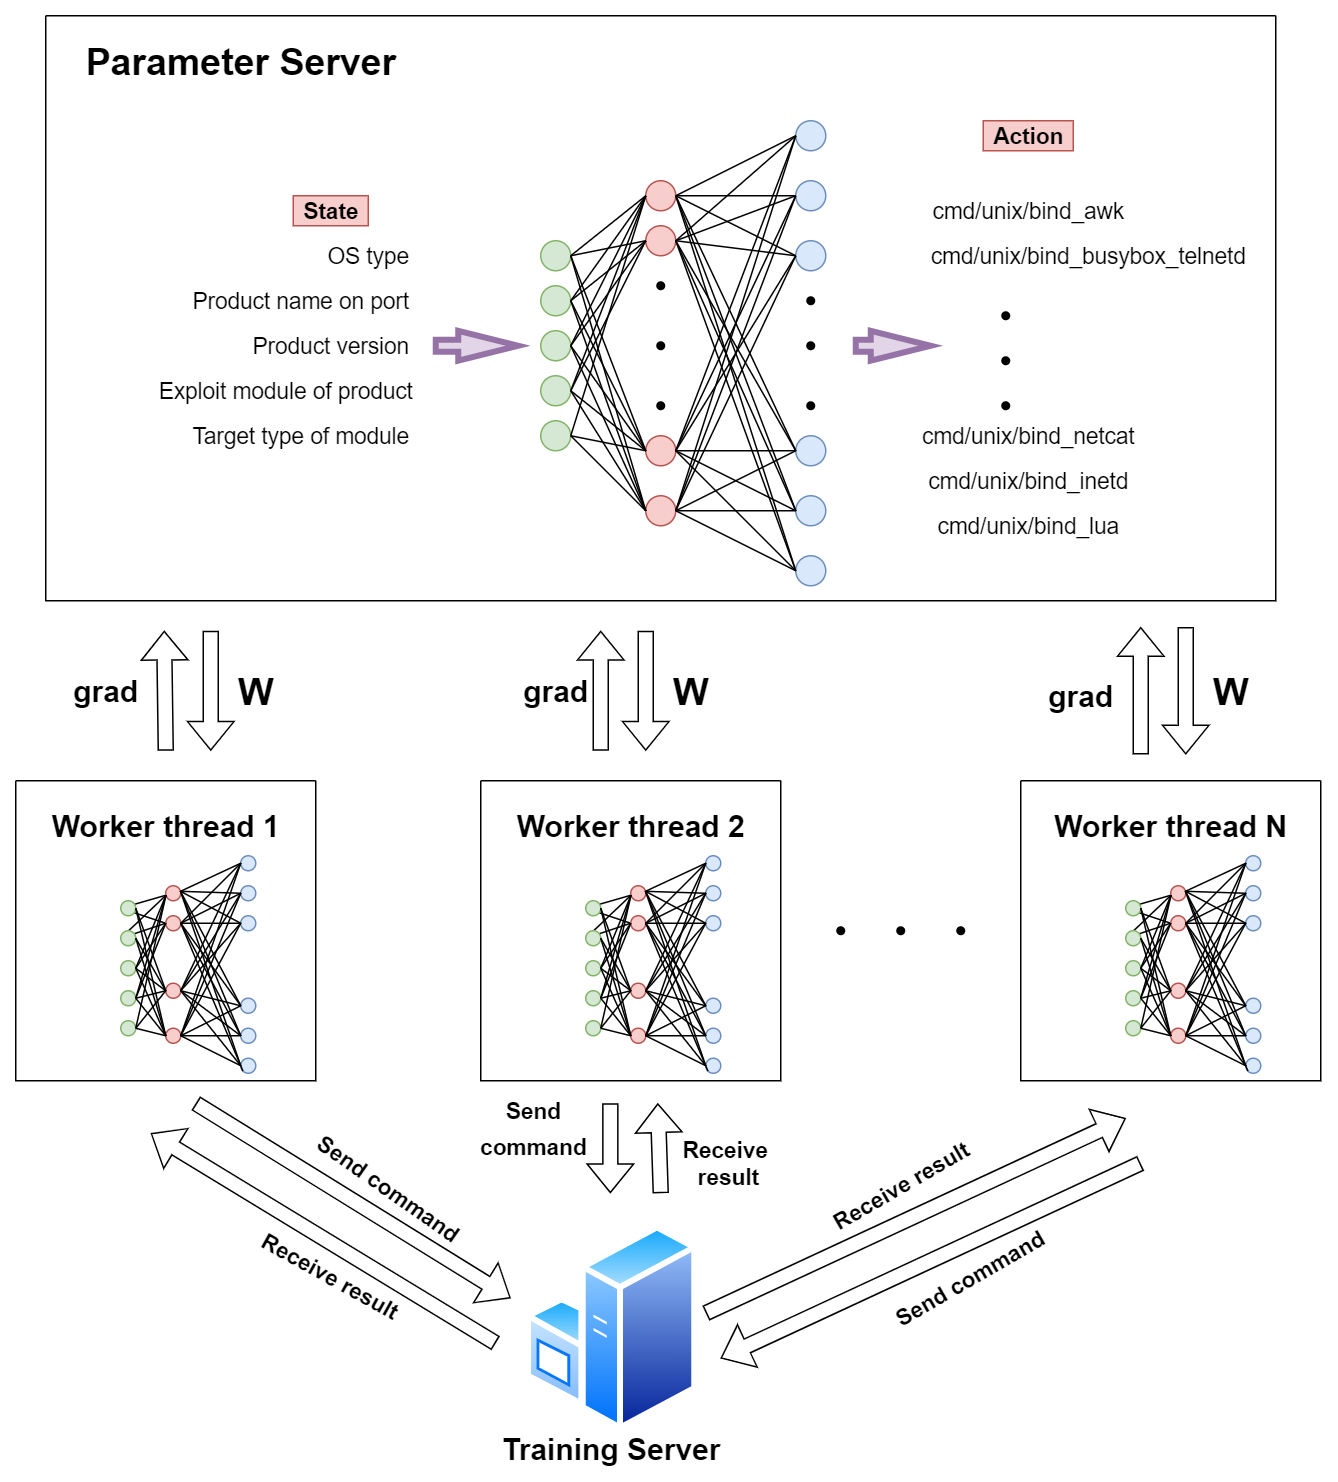
\includegraphics[scale=0.3]{graphics/chapter-3/chap3-RLA3C_AutoPentest.png}
    \caption{Chiến lược học tăng cường sâu với nhiều agent} 
    \label{fig:chap3-RLA3C_AutoPentest}
\end{figure}

Giả sử chúng ta định nghĩa hàm $J(\pi)$ như trong công thức \textbf{(\ref{eq5})}, là một phần thưởng có chiết khấu cho sự khớp trung bình $\pi$ qua tất cả các agent, bắt đầu với trạng thái đầu tiên $s_0$.
\begin{equation}
J(\pi) = E_p(s_0)[V(s_0)]
\label{eq5}
\end{equation}

Để cải thiện con số này, chúng ta cần tính toán độ dốc của $J_{\pi}$ với hàm ưu điểm \textit{A(s,a)}, như trong công thức \textbf{(\ref{eq6})}:
\begin{equation}
\bigtriangledown_{(\theta)}J_{\pi} = E_{s\sim_{\pi},a\sim\pi_{s}} [ A(s,a).\bigtriangledown_{(\theta)} Log \pi(a||s) ]
\label{eq6}
\end{equation}

Trong đó, hàm ưu điểm \textbf{A(s,a)} cho biết lợi ích của việc thực hiện hành động \textit{a} trong trạng thái \textit{s}. $\bigtriangledown_{(\theta)} Log \pi(a||s)$ cho biết một hướng mà xác suất thành công của hành động tăng lên. Cả hai trong những điều này nằm trong kỳ vọng của phân phối trạng thái và hành động của $\pi$. Tuy nhiên, chúng ta không thể tính toán chính xác nó trên mọi trạng thái và mọi hành động. Thay vào đó, chúng ta có thể sử dụng tính chất trung bình của các mẫu với phân phối xác suất. Do đó, chúng ta chỉ cần để agent chạy trong môi trường và ghi lại các mẫu \textit{(s,a,r,s')}. Sau đó, chúng ta sử dụng công thức trên để tìm một xấp xỉ của độ dốc $\bigtriangledown_{(\theta)}J_{\pi}$ và cập nhật chính sách một lần nữa.

Điểm cốt lõi của học tăng cường là thực hiện các hành động chính xác tại các trạng thái đầu vào khác nhau thông qua việc thử - sai dựa trên kết quả của các kinh nghiệm trước đó. Kết quả là, khả năng tự động exploit sẽ chính xác và ít tốn thời gian hơn. Ngoài ra, mỗi luồng công việc hoạt động như một agent Hhọc song song với [PS] - Máy chủ Tham số và [WT] - Luồng Công việc, như được miêu tả trong Hình \textbf{\ref{fig:chap3-RLA3C_AutoPentest}}. Cơ chế học tập của mô hình đã nêu trên được mô tả như sau:

\begin{itemize}
    \item \textbf{Bước 1:} [PS] khởi tạo trọng số mạng (w) với các giá trị ngẫu nhiên.
    \item \textbf{Bước 2:} [PS] sao chép trọng số mạng (w) cho các luồng công việc.
    \item \textbf{Bước 3:} [WT]  nhập trạng thái hiện tại vào mạng và chọn một số hành động.
    \item \textbf{Bước 4:} [WT] nhận phần thưởng cho các hành động. 

Vì trạng thái thay đổi khi một hành động được thực hiện, điều này được gọi là \textbf{"trạng thái tiếp theo"}. 
    \item \textbf{Bước 5:} [WT] lưu một bộ tứ gồm trạng thái hiện tại, hành động, phần thưởng và trạng thái tiếp theo như kinh nghiệm trong bộ nhớ.

    \item \textbf{Bước 6:} [WT] lặp lại các bước 3 đến 5 ở trên.
    \item \textbf{Bước 7:} [WT] sau khi tích lũy một lượng kinh nghiệm nhất định, tính gradient của mạng (grad) bằng cách sử dụng các kinh nghiệm trong bộ nhớ (trạng thái hiện tại, hành động, phần thưởng, trạng thái tiếp theo).
    \item \textbf{Bước 8:} [WT] đẩy grad lên máy chủ tham số. 
    \item \textbf{Bước 9:} [PS] cập nhật trọng số mạng (w) bằng cách sử dụng grad được đẩy từ mỗi luồng công việc. 

    \item \textbf{Bước 10:} Quay lại Bước 2 ở trên.
\end{itemize}

Theo cách này, nhiều tác nhân làm việc không đồng bộ trên các nhiệm vụ và chia sẻ kinh nghiệm của chúng để tăng tốc quá trình học.